\documentclass[../script.tex]{subfiles}
	% Next figure will be labeled fig9
			\begin{corollary}\label{cor20}
				There exists a pseudo-polynomial algorithm for Partition.
			\end{corollary}
			\begin{proof}
				Use the algorithm for Subset Sum with $K\coloneqq \frac{1}{2}\sum_{i=1}^n a_i$.
			\end{proof}

			\begin{definition}
				An NP-complete (NP-hard) problem is called \textbf{strongly} NP-complete (\textbf{strongly} NP-hard), if there exists some polynomial $p$ s.t. the problem stays NP-complete (NP-hard), if restricted to instances with $Max(x)\leq p(|x|)$
			\end{definition}

			\begin{theorem}[Garey, Johnson 1978]\label{thm21}
				Unless P=NP, there does not exist an exact pseudo-polynomial algorithm for any strongly NP-hard problem. 
			\end{theorem}

			\begin{corollary}\label{cor22}
				Integer Linear Inequalities is strongly NP-complete.
			\end{corollary}
			\begin{proof}
				See proof of \cref{thm11}: All numbers in the reduction were in $\{-1,0,1\}$.
			\end{proof}

		\subsection{Simple Max Cut}
			\textbf{Input:} A graph $G=(V,E), K\in\mathbb{N}$\par
			\textbf{Question:} Is there an $S\subseteq V$ s.t. $|\delta(S)|\geq K$?
			\begin{theorem}[Garey, Johnson, Stockmeyer 1976]\label{thm23}
				Simple Max Cut is NP-Complete.
			\end{theorem}

			\begin{corollary}\label{cor24}
				Max Cut is strongly NP-complete.
			\end{corollary}

			\begin{proof}[Proof of \cref{thm23}]
				Obviously the problem is in NP.
				Reduction from Stable Set:\par
				Let $G=(V,E),K$ be an instance of stable set. Construct a graph $G'= (V',E')$ as follows:\par
				\begin{eqnarray*}
					V' &\coloneqq& V\cup\{x\}\cup\bigl\{ \{e,i\}|\,e\in E(G), i=1,2 \bigr\}
				\end{eqnarray*}
				\begin{figure}[ht]
					\centering
					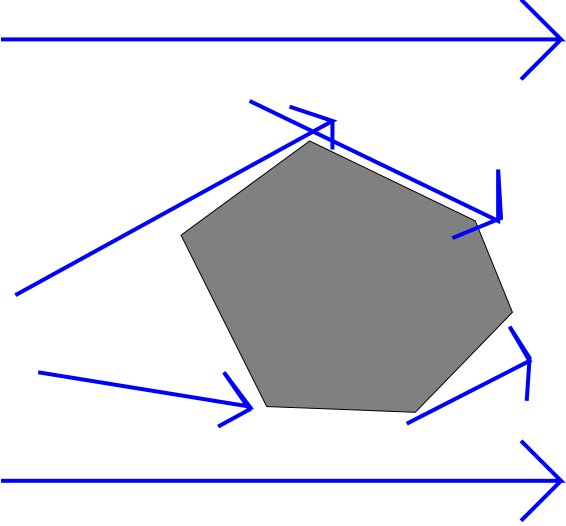
\includegraphics[width=0.4\textwidth]{Images/app9.png}
					\caption{The way $E'$ is defined shown in a picture}
					\label{fig9}
				\end{figure}
				Definition of $E'$ by picture in \cref{fig9}
				\begin{figure}[ht]
					\centering
					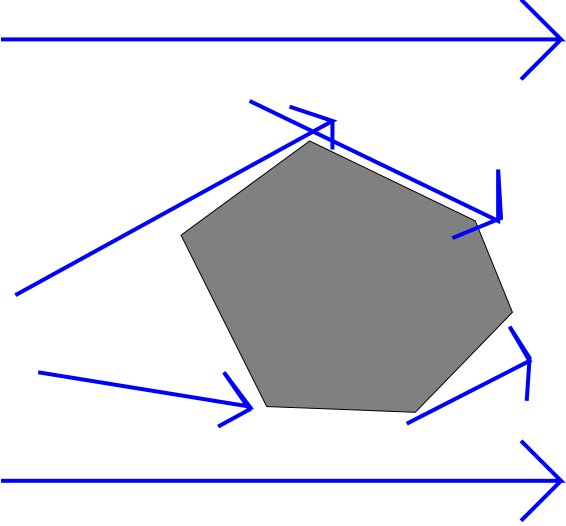
\includegraphics[width=0.4\textwidth]{Images/app10.png}
					\caption{Cuts created. In each case we have 5 additional vertices}
					\label{fig10}
				\end{figure}
				\textbf{Claim:} $G$ has a stable set of size $K \Leftrightarrow G'$ has a cut with $K+4|E|$ edges.\par
				$``\Rightarrow''$ $S$ is a stable set of size $K$. Add the vertices $(e,1), (e,2)$ appropriately, s.t. 4 edges of the edge gadget are cut. $\Rightarrow$ $4|E| + K$ edges.\par
				$``\Leftarrow''$ For each edge-gadget at most $4$ edges are in the cut $\Rightarrow$ at least $K$ edges of the form $\{x,v\}$ are in the cut
				\[
					S_C\coloneqq \{v\in V|\,\{x,v\}\in\text{ cut}\},\quad |S_C| = K+\ell,\quad \ell\geq 0
				\]
				so $\leq \ell$ edges for which only 3 edges of the edge gadget are in the cut. For each such edge ($3$ edges in the edge gadget) remove one of the endpoints from $S_C$ and call the remaining vertices $S$. Then $S$ is a stable set and
				\[
					|S|\geq |S_C| - \ell = K+\ell-\ell = K.
				\]
			\end{proof}

			\textbf{Conclusion:} We have seen that for some of the ``easy'' problems, a pseudo-polynomial time algorithm exists.

\chapter{Approximation Algorithms}\label{c3}
	In this example we will give some example of Approximation Algorithms.
	\begin{definition}
		An \textbf{Approximation Algorithm} $A$ for an optimization problem $P$ is a \emph{polynomial time} algorithm for $P$. $A$ has \textbf{approximation ratio} $c$, if (for $c\in\mathbb{R}$) we have
		\begin{IEEEeqnarray*}{rCl}
			A(I) &\leq& c\cdot OPT(I)\quad\text{if }P\text{ is a minimization problem}\\
			A(I) &\geq& c\cdot OPT(I)\quad\text{if }P\text{ is a maximization problem}
		\end{IEEEeqnarray*}
		If $P$ is a minimization problem we assume $1\leq c\leq\infty$ and if $P$ is a maximization problem then $0\leq c\leq 1$ holds.
	\end{definition}

	\section{Minimum Weight Set Cover Problem}
		\textbf{Input:} A family $S_1,...,S_m$ of subsets of a finite set $U$ with $\bigcup_{i=1}^n S_i = U,\,c:\{S_1,...,S_m\}\to\mathbb{R}_+$\par
		\textbf{Output:} A subfamily $S_{i_1},...,S_{i_k}$ s.t. $\bigcup_{j=1}^k S_{i_j} = U$ s.t.
		\[
			\sum_{j=1}^k c(S_{i,j}) 
		\]  
		is minimal.

		\subsection*{Greedy Weighted Set Cover Algorithm}
			\textbf{Input:} $S_1,...,S_m,U,\bigcup S_i = U, c:\{S_1,...,S_m\}\to\mathbb{R}_+$\par
			\textbf{Output:} Optimum subfamily $E$ of the $S_i$
			\begin{itemize}
				\item $C\coloneqq\emptyset$, $E\coloneqq\emptyset$
				\item while $C\neq U$
				\item TAB choose $S\in\{S_1,...,S_m\}$ s.t. $\frac{c(S)}{|S\setminus C|}$ is minimum
				\item TAB $C\coloneqq C\cup S$
				\item TAB $E\coloneqq E\cup{S}$
			\end{itemize}

			\begin{theorem}\label{thm23}
				The greedy weighted set algorithm has approximation ratio
				\[
					H_n\coloneqq \sum_{i=1}^n \frac{1}{i},\quad\text{if } n\coloneqq |U|.
				\]
			\end{theorem}
			\begin{proof}
				W.l.o.g assume $E=\{S_1,...,S_k\}$ (i.e. we order our sets in a way s.t. the algorithm returns the first $k$ of them). For each $x\in U$ assign cost
				\[
					\tilde c(x)\coloneqq \frac{c(S_i)}{|S_i\setminus\{S_1\cup...\cup S_{i-1}\}},
				\]
				where $i$ is chosen minimum s.t. $x\in S_i$.\newline\newline\noindent
				\textbf{Claim:} For $S\in\{S_1,...,S_m\}$ we have
				\[
					\sum_{x\in S} \tilde c(x) \leq c(S)\cdot H_{|S|}.
				\]
				If we prove this claim we are done: Let $E^*$ be an optimum solution. Then
				\begin{IEEEeqnarray*}{rCl}
					\sum_{S\in E} c(S) &=& \sum_{x\in U}\tilde c(x) \\&\leq& \sum_{S\in E^*}\sum_{x\in S}\tilde c(x)\\
					&\overset{\text{claim}}\leq&\sum_{S\in E^*}c(S)\cdot H_{|S|} \leq H_n\cdot\sum_{S\in E^*}c(S).
				\end{IEEEeqnarray*}
				\textbf{Proof of the claim:} Let $S=\{x_1,...,x+p\}\in \{S_1,...,S_m\}$ s.t. $x_i$ is covered not earlier than $x_j$, if $i\geq j$. Consider the step where the greedy algorithm covers $x_i$ for the first time, $1\leq i\leq p$. The greedy algorithm could have chosen $S$. We know for sure that
				\begin{IEEEeqnarray*}{rCl}
					\tilde c(x_i) \leq \frac{c(S)}{|S|-(i-1)}.
				\end{IEEEeqnarray*}
				Therefore
				\begin{IEEEeqnarray*}{rCl}
					\sum_{x\in S}\tilde c(x) &\leq& \sum_{i=1}^{|S|} \frac{c(S)}{|S|-(i-1)}\\
					&=& c(S)\sum_{i=1}^{|S|}\frac{1}{i}\\
					&=& c(S)H_{|S|},
				\end{IEEEeqnarray*}
				and this is the claim.
			\end{proof}

			\begin{remark}
				From the proof we get a slightly stronger statement, namely that
				\[
					\sum_{S\in E}c(S) \leq H_{\max_{S\in\{S_1,...,S_m\}}|S|}\sum_{S\in E^*}c(S).
				\]
				We also observe that the runtime is polynomial, namely it is 
				\[
					O\left(m^2 + \sum |S_i|\right)
				\]
			\end{remark}
			\textbf{The Analysis is best possible: } Take a set of $n$ elements and take a singleton set for each element. Assign the weight $\frac{1}{n-(i-1)}$ for the singleton set $i$ (assign the weight $1+\varepsilon$ to the whole set). Then the approximation ratio is $\frac{H_n}{1+\varepsilon}$. Even in the unweighted case, there is an example with 12 sets that shows that the analysis was best possible.\newline\newline\noindent

			\textbf{Question: } What happens if $c:\{S_1,...,S_m\}\to\mathbb{R}$, i.e. negative weights for some sets are possible?\par
			An idea would be to take all sets with negative weight and run the greedy algorithm on the remaining algorithms. This has approximation ratio $\infty$. \newline\newline\noindent
			\begin{remark}An interesting case for the problem is if $|S_i|\leq 2$. Then this is an edge cover problem (in P). Already for a bound of $3$, the problem becomes NP-hard. \end{remark}

	\section{Vertex Cover: Special case of set Cover}
		\begin{theorem}\label{thm24}
			There exists a $2$-approximation for \emph{Minimum Vertex Cover}.
		\end{theorem}
		\begin{proof}
			Compute a maximal matching and take all endpoints of the matching into a set $S$. Then $S$ is a vertex cover of size $\leq 2 OPT$.\newline\newline\noindent
			\textbf{Observation: } For each matching edge at least one endpoint must be in a vertex cover.
		\end{proof}

		Unless P=NP $1.36$ is a lower bound on the approximation ratio. One doesn't know yet whether a better constant exists.

	\section{$k$-Center}
		\textbf{Input:} A finite set $X$, a metric $dist:X\times X\to\mathbb{R},K\in\mathbb{N}$\par
		\textbf{Output:} A set $C\subseteq X$ with $|C|=K$ s.t. $\max_{x\in X}\min_{c\in C}dist(x,c)$ is minimum\newline\newline\noindent
		$k$-Center can be solved in $O(k|X|^{k+1})$, i.e. we have polynomial runtime if $k = const$.\newline\newline\noindent
		Consider $X$ to be the vertices of a complete graph. Then We can identify the metric with $dist:E(G)\to\mathbb{R}_+$.
		\begin{definition}
			Given a graph $G=(V,E)$ one says that $D\subseteq V(G)$ is a \textbf{dominating set} if for all $v\in V(G)\setminus D$ there is some $d\in D$ with $\{v,d\}\in E(G)$. The \textbf{domination number} of the graph is defined as
			\[
				dom(G)\coloneqq \min\{|D|:\,D\text{ is a dominating set in} G\}.
			\]
		\end{definition}
		